\section{Results}
\label{sec:results}
In this section, we present the results in the order of the processing chain. We first analyze the recognition of a single sonar view, and how far a robot may deviate from a template for it still to be recognized. Next, we evaluate the complete system, followed by ablations, a robustness analysis and the computational cost.

\subsection{Sonar Template Recognition}
\label{sec:resultsFrontend}
To evaluate the front-end on its own, we tested how well a single local view recognizes the place where it was taken, without the sequence verifier. For every third pulse, we compared its local view with those of all earlier pulses at least \SI{6}{\meter} of travel back, using the similarity of equation \ref{eq:similarity}. Only pulses with a true revisit, i.e., an earlier pulse within \SI{0.6}{\meter} and \SI{26}{\degree}, serve as queries, so that only same-direction revisits are counted. We report two metrics. The \emph{top-1 accuracy} is the fraction of queries for which the most similar earlier view lies within \SI{1}{\meter} and \SI{30}{\degree} of the query. The \emph{AUC} is the area under the ROC curve that separates same-place pairs (within \SI{0.6}{\meter} and \SI{26}{\degree}) from different-place pairs (more than \SI{3}{\meter} or \SI{57}{\degree} apart), i.e., the probability that a random same-place pair is more similar than a random different-place pair. We estimate it from 20\,000 random pairs of each class, so that differences in AUC below about 0.005 lie within its sampling noise. Figure \ref{fig:sensor} reports both metrics for different sensors, and table \ref{tab:descriptor} in the appendix for the design choices of the descriptor.

\textbf{Sensor quality:} Figure \ref{fig:sensor} compares four sensors on the same drive through the city map, combining two maximal ranges (\SI{5}{\meter} and \SI{10}{\meter}) with two noise levels (\SI{-96}{\deci\bel} and \SI{-116}{\deci\bel}, i.e., the standard deviation of the noise relative to the peak amplitude of the emitted call). For every sensor, we evaluated three descriptors: the descriptor of the original BatSLAM (8 frequency channels, \SI{3}{\centi\meter} range bins and a logarithmic compression with a floor at \SI{-30}{\deci\bel}), the same with the time-varying gain (TVG), and our final descriptor (section \ref{sec:frontend}). The noise level clearly dominates. At a noise level of \SI{-96}{\deci\bel}, no descriptor reaches a top-1 accuracy of 0.5, and a longer range does not help, as the echoes beyond \SI{5}{\meter} are buried in noise. The TVG then even hurts, as it amplifies this noise, and the final descriptor offers no clear advantage over the original one. With \SI{20}{\deci\bel} less noise (\SI{-116}{\deci\bel}), every descriptor improves substantially, and both the TVG and the final descriptor pay off. Only then does a longer range pay off as well, up to a top-1 accuracy of \SensorTopOneBest{} for the final descriptor at \SI{10}{\meter}. This sensor (\SI{10}{\meter}, \SI{-116}{\deci\bel}) is the design sensor that we use in the remainder of this paper. To test the robustness, we also use three degraded sensors: the design sensor with \SI{10}{\deci\bel} and \SI{20}{\deci\bel} more noise (the \SI{-10}{\deci\bel} and \SI{-20}{\deci\bel} sensors, at \SI{-106}{\deci\bel} and \SI{-96}{\deci\bel}), and the sensor of the original configuration (\SI{5}{\meter}, \SI{-96}{\deci\bel}).

\begin{figure*}[t]
\centering
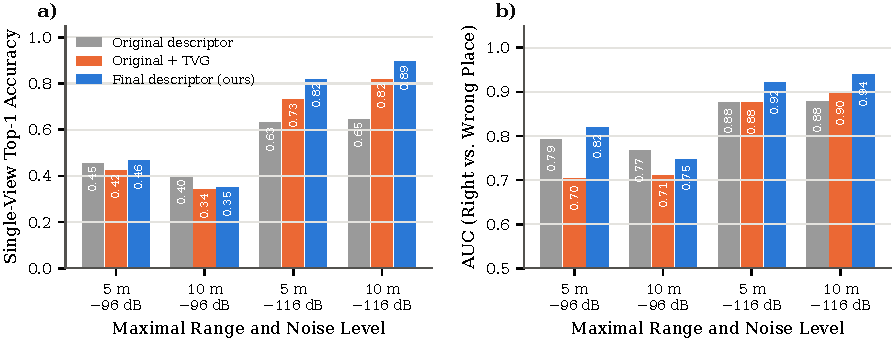
\includegraphics[width=\linewidth]{figures/recognitionSensor.pdf}
\caption{Single-view place recognition for four sensors on the city drive: a) top-1 accuracy, b) AUC. Grey: descriptor of the original BatSLAM; orange: the same with TVG; blue: the final descriptor.}
\label{fig:sensor}
\end{figure*}

\textbf{Descriptor design:} Table \ref{tab:descriptor} in the appendix compares the design choices of the descriptor for the design sensor on both worlds. All variants share the spatiospectral resolution (32 frequency channels, \SI{6}{\centi\meter} range bins) and the TVG of our front-end, and differ only in the listed aspect. Adding the spectral-shape image to the energy image raises the top-1 accuracy on the indoor floor from \TopOneEnergyIndoor{} to \TopOneFinalIndoor{}, and the AUC on both worlds. Adding the interaural level difference (ILD) as a third image raises the AUC further, but lowers the top-1 accuracy on both worlds, as the ILD changes quickly with small pose changes, and we therefore left it out. The compression law matters little: with the spectral-shape image, every compressive law reaches a top-1 accuracy between 0.88 and 0.93 on the indoor floor and of 0.89 in the city, and only a linear amplitude is clearly worse. We use the cube root, as it performs on par with a logarithm without a floor that depends on the noise level (section \ref{sec:frontend}). The matching method, in contrast, has shown to matter a lot. With the matching of the original BatSLAM (the Euclidean distance between unit-energy views, without range shift), the top-1 accuracy of our descriptor drops to about 0.80 on both worlds, and that of a logarithmic energy image alone to 0.40 and 0.60. Both the new descriptor and the new matching thus contribute to the improvement over the original BatSLAM. Note that these last rows use the resolution and TVG of our front-end, and therefore differ from the original descriptor in figure \ref{fig:sensor}.

\subsection{Capture region of a view template}
\label{sec:resultsCapture}
To measure how far a revisit may deviate from a template, we rendered views at controlled offsets from 16 template poses along the development drive. An offset view counts as recognized when its similarity to the template exceeds \LLRmid{} and no template of another place is more similar. Figure \ref{fig:capture} shows that the capture region is narrow: about \CaptureAlong{} along track, \CaptureLateral{} laterally and \CaptureHeading{} in heading. 

\begin{figure}[t]
\centering
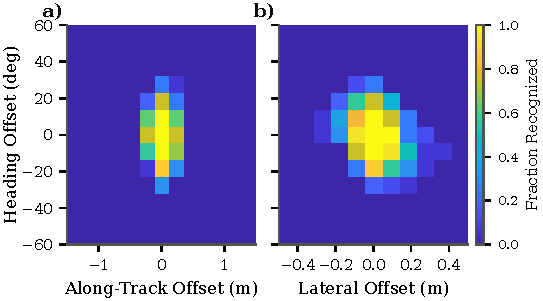
\includegraphics[width=\linewidth]{figures/captureRegion.pdf}
\caption{Capture region of local view templates on the indoor floor, averaged over 16 template poses: fraction of recognized offset views for combined a) along-track and heading offsets, and b) lateral and heading offsets.}
\label{fig:capture}
\end{figure}

\subsection{The complete system}
\label{sec:resultsMain}
We ran the complete system on three odometry seeds of the development drive, the two unseen routes and the city environment (which was unseen during development), each with calibrated odometry and with a residual heading bias, on three degraded sensors, and with uncalibrated odometry. Table \ref{tab:main} in the appendix summarizes the results per condition, figure \ref{fig:worlds}d--f shows the maps of one run per world, figure \ref{fig:loopmatrix} shows the links of one run, and table \ref{tab:mainRuns} and figure \ref{fig:appendixMaps} in the appendix list all runs.

With the design sensor and calibrated or roughly calibrated odometry, all \NdesRuns{} runs produced a consistent map: none of the \CommitsDes{} committed hypotheses was wrong, and no distant places were pulled together. The link precision was \PrecDesRange{}, and \CovDesRange{} of the true revisits were linked. The trajectory error was \ATEdesRange{} (\ATEalignedDesRange{} after alignment), against \ATEodoDesRange{} for odometry alone.

The degraded sensors also produced consistent maps (\ATEalignedDegRange{} after alignment), but on the \SI{-20}{\deci\bel} sensor, one wrong hypothesis of 17 links survived. It was committed early in the drive, when the map was still so uncertain that a correction of \SI{8}{\meter} was plausible, and it distorts the map locally without collapsing it.

The difference between the aligned and unaligned errors is caused by the heading drift that accumulates before the first loop closure, which can only be removed by a later loop closure with that first stretch of the route. If there is none, the whole map remains rotated (by about \SI{5}{\degree} on route 7). The unaligned error therefore measures how the map is anchored, and the aligned error measures its shape. With uncalibrated odometry, the links remain almost all correct, but the metric accuracy degrades (section \ref{sec:resultsRobust}).

\begin{figure}[t]
\centering
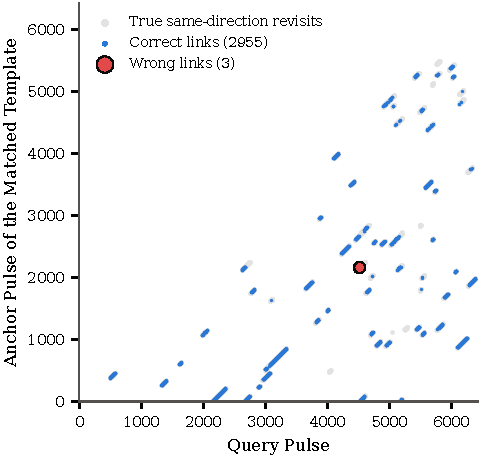
\includegraphics[width=0.92\linewidth]{figures/loopMatrix.pdf}
\caption{Loop closure matrix of the development drive (route 3, calibrated odometry). Every dot is a link in the final graph between a query pulse and the anchor of the matched template. Grey: true same-direction revisits; blue: correct links; red: wrong links.}
\label{fig:loopmatrix}
\end{figure}

\subsection{Ablations}
\label{sec:resultsAblation}
To assess the contribution of every component, we removed or replaced several components of the full system, one at a time, and evaluated all variants on four standard cases (tables \ref{tab:ablation} and \ref{tab:ablationCases} in the appendix). Without sequence verification, the system made 215 wrong commits, of which 10 survived the link management, and the mean trajectory error grew to \SI{4.85}{\meter}. Without link management as well (the naive variant), the map collapsed completely (rendering ATE a useless metric). This confirms that a single sonar view is too ambiguous to be trusted to perform loop closure. The front-end matters has an equally large contribution to the performance of the system, as removing the time-varying gain or the spectral-shape image, wrong hypotheses survive often. Without the range-shift search, the coverage of recognition drops to 0.60. The original front-end and the hand-set evidence constants of our first implementation made no wrong commits, but linked fewer revisits (0.73 and 0.68).

The safeguards against aliases, in contrast, hardly come into play on these cases, as they contain almost no aliases that survive the sequence verification. Removing the complete link management even lowered the error (\SI{0.55}{\meter} against \SI{0.87}{\meter}), as the length rule also withdraws short correct groups. Requiring 24 pairs for a large correction, without a condition on the evidence, raised the error on one particular run to \SI{2.98}{\meter}, as the true revisit of the start of the route was split into two hypotheses that never reached 24 pairs, which left the map rotated.

\textbf{Safeguards against aliases:} To study the safeguards, we repeated the ablations on the four hardest cases: the three degraded sensors and a development drive with a recurring alias (table \ref{tab:ablationHard} in the appendix). Without the risk-scaled commit, 12 of 346 commits were wrong. Of these, 8 implied a correction of more than \SI{1.5}{\meter} (against only \SI{13}{\percent} of the correct commits), and 11 ended with 16 links or fewer, as an alias ends where the similarity between both corridors does. These observations motivate the risk-scaled commit and the length rule. With all safeguards in place, 6 wrong hypotheses were committed, and the link management withdrew all but the early alias on the \SI{-20}{\deci\bel} sensor. Without link management, 7 survived, and removing only the length rule gave identical results: the residual check and GNC audits never changed a final map, as a single wrong hypothesis that passed the gates of the verifier cannot be detected by a joint consistency test. Without any plausibility gate, 3 wrong hypotheses survived. Requiring 24 pairs regardless of the evidence is the only variant without a surviving wrong hypothesis, but as shown above, it also withholds the loop closures that anchor the map (section \ref{sec:limitations}).

\subsection{Robustness}
\label{sec:resultsRobust}
Next, we varied the systematic odometry error with the bias factor $b$, tripled the random odometry noise, and combined the degraded sensors with a residual bias (figure \ref{fig:robustness}; table \ref{tab:robustness} in the appendix). Up to $b = 0.5$ (\SI{0.3}{\degree\per\meter}), every run produced a consistent map with the same coverage as with calibrated odometry, while the error of dead reckoning grew beyond \SI{20}{\meter}. The same holds for three times the random noise (\SI{0.48}{\meter} after alignment). With uncalibrated odometry ($b = 1$), the heading has drifted by about \SI{45}{\degree} at the first revisit. In three of six runs, later loop closures removed this rotation (\SI{1.4}{\meter} to \SI{1.8}{\meter}). In the other three, the links were still correct, but as the pose graph treats odometry errors as random, the stretches between loop closures keep the curvature of the biased odometry, and the map remains distorted (\SI{9.3}{\meter} to \SI{14.5}{\meter}). With $b = 2$, fewer true revisits pass the consistency test and plausibility gate (coverage 0.32 to 0.41), and the map collapses about as much as dead reckoning does, but not a single wrong hypothesis remained. In summary, BatSLAM 2.0 needs odometry calibrated to within about \SI{0.3}{\degree\per\meter}, and beyond that, it degrades in metric accuracy rather than in topology.

\begin{figure*}[t]
\centering
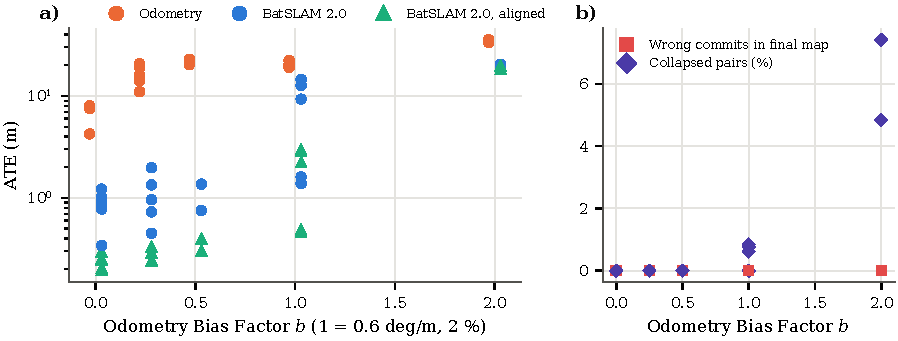
\includegraphics[width=\linewidth]{figures/robustness.pdf}
\caption{Robustness against systematic odometry errors on the development drive. a) Trajectory error of odometry (orange), BatSLAM 2.0 (blue) and BatSLAM 2.0 after alignment (green) versus the bias factor $b$; b) wrong hypotheses in the final graph and percentage of collapsed pairs.}
\label{fig:robustness}
\end{figure*}

\subsection{Computational cost}
\label{sec:resultsCost}
On a single core, a pulse took \SI{\CostTotal}{\milli\second} on average, of which \SI{\CostGraph}{\milli\second} went to the pose graph. As the template comparison and the pose graph grow with the map, our (unoptimized) Python implementation meets the \SI{100}{\milli\second} budget of a \SI{10}{\hertz} pulse rate on average, but not towards the end of a \SI{1}{\kilo\meter} drive.
